% arara: pdflatex
\documentclass{beamer}
\usepackage[utf8]{inputenc}

\title{\Huge\texttt{vim} \\ \normalsize ``Who needs a mouse?''}
\author{Nicolas Dorrmann}
\date{04. Nov. 2020}

\begin{document}
\frame{\titlepage}

\begin{frame}
    \frametitle{History and Design Philosophy}
    \begin{itemize}
        \item Developed by Bram Moolenaar, initially released in 1991.
        \item Successor to \texttt{vi} (\textbf{v}isual \textbf{i}nterface for line editor \texttt{ex}).
        \item Editing works entirely over keyboard, most commands are easily reachable over home row.
        \item Plugins (written in \texttt{VimScript}) \textit{can} provide functionality similar to an IDE.
    \end{itemize}
\end{frame}
\begin{frame}
    \frametitle{Basics}
    \begin{itemize}
        \item Modes
            \begin{description}
                \item [\texttt{NORMAL}]  navigate within the file, issue text commands (yank/change/delete)
                \item [\texttt{COMMAND}] open, close, or save a file
                \item [\texttt{INSERT}]  direct input (i.\ e.\ actually typing text)
                \item [\texttt{VISUAL}]  text highlighting, text blocking
            \end{description}
    \end{itemize}
    \vspace{0.5cm}
    \begin{center}
        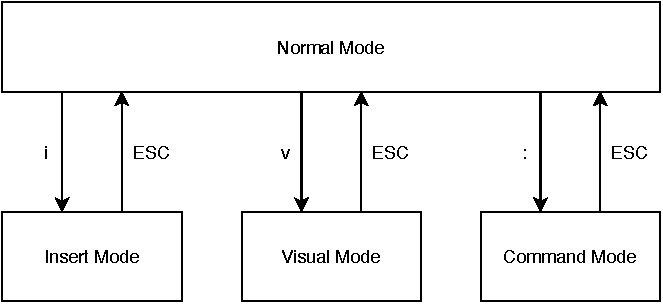
\includegraphics[width=0.6\textwidth]{vim_modes.pdf}
    \end{center}
\end{frame}
\begin{frame}
    \frametitle{Basics}
    \begin{itemize}
        \item Text Objects
            \begin{description}
                \item [word]      string of non-whitespace characters surrounded by whitespace
                \item [sentence]  ends with \texttt{!}, \texttt{?}, \texttt{.} followed by newline
                \item [paragraph] consists of several sentences, delimited by empty lines
            \end{description}
    \end{itemize}
\end{frame}
\end{document}

